% Template para la realización de la Presentacion de la Tesis.

% Tipo de Documento.
\documentclass[a4paper]{article}

% Idioma.
\usepackage[utf8x]{inputenc}
\usepackage[spanish]{babel}
\usepackage{babelbib}

% Margenes.
\usepackage[outer=4cm,inner=2cm,top=2cm,bottom=2cm]{geometry}
\usepackage{fancyhdr}
\usepackage{lastpage}

% Graficos.
\usepackage{graphicx}
\graphicspath{{./images/}}

% Codigo Fuente.
\usepackage{tabularx}

% Hypervinculos.
\usepackage{url}
\usepackage{color,hyperref}
\definecolor{black}{rgb}{0.0,0.0,0.0}
\definecolor{darkblue}{rgb}{0.0,0.0,0.3}
\hypersetup{colorlinks,breaklinks,
            linkcolor=black,urlcolor=darkblue,
            anchorcolor=darkblue,citecolor=darkblue}

% Guiones
\hyphenation{pro-ble-ma}
\hyphenation{ge-ne-ra-ra}
\hyphenation{pos-te-rior-men-te}

% Definicion de la hoja de firmas.
\newcommand{\signature}[7]{
   \vfill

   \begin{flushright}
      #1, \today
   \end{flushright}
   \vspace{3cm}

   \noindent
   \centering
   \begin{tabularx}{0.9\textwidth}{cXc}
      \multicolumn{3}{c}{\rule{5cm}{1pt}}\\
      \multicolumn{3}{c}{#2}\\
      \multicolumn{3}{c}{#3}\\
      \vspace{3cm}\\
      \rule{5cm}{1pt} & \hspace{2.5cm} & \rule{5cm}{1pt} \\
      #4 & ~ & #5 \\
      #6 & ~ & #7
   \end{tabularx}
   \vspace{1cm}
}

% Encabezado y Titulo del Documento y de la Tesis.
\title{
   {\normalsize
      Universidad de Buenos Aires\\
      Facultad de Ingeniería -- Departamento de Electrónica\\
      Propuesta de Tesis de Ingeniería Electrónica\\
      \vspace{0.7cm}
   }
   Implementación de una Unidad de Punto Flotante basado en el algoritmo BKM
}

% Datos de autor: Tesista, Director y Co-director.
\author{ \textbf{Tesista}                                                           \\
         Ignacio Lesser, \textit{Padrón Nro. 90.942}                                \\
         \texttt{ \href{mailto:ignacio.lesser@gmail.com}{ignacio.lesser@gmail.com}}  \\[2.5ex]
         \textbf{Director}                                                          \\
         Ing. Nicolas Alvarez, \textit{Profesor Adjunto}                            \\
         \texttt{ \href{mailto:nalvare2001@yahoo.com.ar}{nalvare2001@yahoo.com.ar}} \\[2.5ex]
         \textbf{Co-director}                                                       \\
         Ing. Octavio Alpago, \textit{JTP. Interino}                                \\
         \texttt{ \href{mailto:oalpago@gmail.com}{oalpago@gmail.com}}               \\[2.5ex]
       }

% Fecha.
\date{\today}

% Pie de Pagina.
\pagestyle{fancy}
\lhead{}
\chead{}
\rhead{}
\lfoot{}
\cfoot{
   {\footnotesize
   \emph{Implementación de una Unidad de Punto Flotante basada en el algoritmo BKM}\\
   Plan de Tesis -- Página \thepage\ de \pageref{LastPage}
   }
}
\rfoot{}
\renewcommand{\headrulewidth}{0pt}
\renewcommand{\footrulewidth}{0.4pt}

% Documento.
\begin{document}

\maketitle

%\thispagestyle{empty}

%\begin{abstract}
%\end{abstract}

\thispagestyle{fancy}

\section{Objeto y Área de la Tesis}

El objetivo principal de este trabajo consiste en diseñar e implementar en hardware digital una unidad de punto flotante basada en el algoritmo BKM. Dicho diseño e implementación será realizado a través del uso del lenguaje de descripción de hardware Verilog, y su síntesis en un dispositivo FPGA \footnote{\label{FPGA}Field Programmable Gate Array: dispositivo semiconductor que contiene bloques de lógica cuya interconexión y funcionalidad puede ser configurada `in situ' mediante un lenguaje de descripción especializado.}.
El interés en este desarrollo proviene de la necesidad de crear un unidad de punto flotante eficiente 

El interés en este desarrollo proviene de la iniciativa de implementar una de las aplicaciones prácticas más importantes de este algoritmo en el área de las comunicaciones digitales. La misma, consiste en la utilización de una técnica de filtrado, que permite la distinción de una señal deseada y el ruido de fondo en un sistema de múltiples antenas, conocida como Beamforming Adaptativo. Este trabajo se da en el contexto de un área de investigación focalizada en el diseño de un sistema Software Defined Radio \footnote{\label{SDR}Software Defined Radio: Sistema de comunicaciones donde los componentes típicamente implementados en hardware (mezcladores, filtros, amplificadores, moduladores / demoduladores, detectores, etc) son implementados en software,}.
El interés en este desarrollo proviene de la necesidad de implementar operaciones matem\'aticas complejas en tiempo real.

El área profesional de relevancia de la presente tesis es el diseño de sistemas digitales y su aplicación en el ámbito de las telecomunicaciones, así como también la aplicación práctica en hardware de algoritmos de procesamiento de señales utilizados en las comunicaciones inalámbricas.

\newpage

\section{Introducción. Antecedentes}

Un \textit{beamformer adaptativo} es un dispositivo que tiene la capacidad de separar señales en el dominio del espacio. Este hecho provee un medio para separar la señal deseada de señales de interferencia. Un \textit{beamformer adaptativo} logra optimizar automáticamente el patrón de un arreglo de múltiples antenas al ajustar el control de los pesos de ponderación hasta que se satisface una determinada función de objetivo preestablecida. Los medios por los cuales esta optimización es lograda están especificados por un algoritmo diseñado para tal propósito. Estos dispositivos utilizan mucha más información disponible en la antena con respecto a un \textit{beamformer} convencional.

\begin{figure}[htb!]
        \centering
        %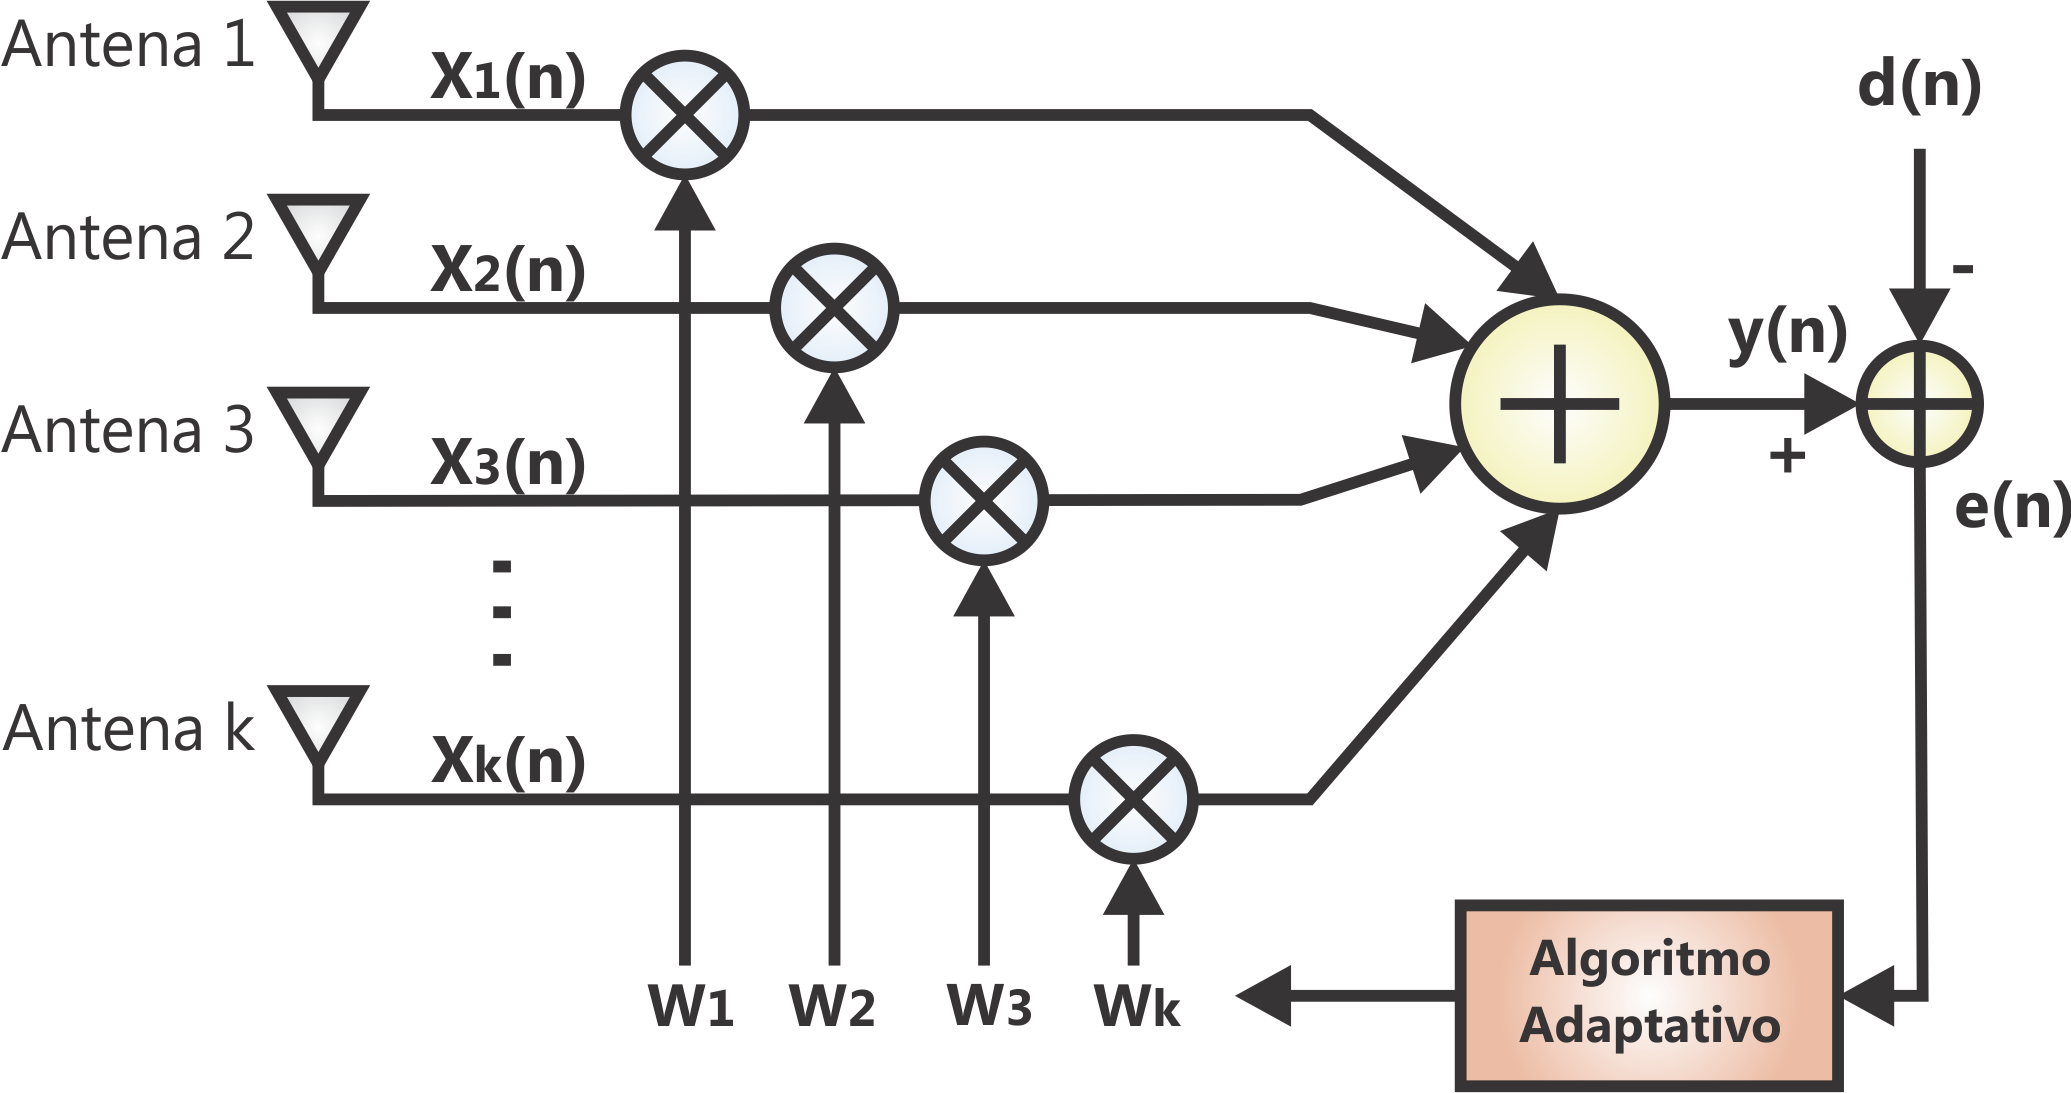
\includegraphics[width=10cm]{adaptive_beamforming.png}
        \caption{Esquema de un sistema de Beamforming Adaptativo}
        \label{fig:Adaptive_Beamforming}
\end{figure}

La elección de algoritmos adaptativos para derivar los pesos adaptativos (o el vector de pesos) es muy importante, dado que determina tanto la velocidad de convergencia como la complejidad de hardware requerida para implementar el algoritmo. Existen dos algoritmos muy populares para resolver esta necesidad, el algoritmo LMS (Least Mean Squares) y el algoritmo RLS (Recursive Least Squares), entre otros.

\subsection{Resolución del algoritmo RLS}

El algoritmo RLS estándar requiere el cómputo explícito de una matriz de correlación. Este es un cálculo intensivo que tiene el efecto de elevar al cuadrado el número de condición del problema, causando un efecto negativo en la longitud de palabra para la estabilidad en sistemas de longitud de palabra finita. Los pesos pueden ser calculados en un modo más estable, evitando el cálculo de la matriz de correlación y su inversa al utilizar la \textbf{Descomposición QR}, una forma de triangularización ortogonal con buenas propiedades numéricas. 

La elección de la implementación utiliza RLS-QRD (algoritmo RLS a través de descomposición QR) como el sistema central para calcular adaptativamente los pesos del filtro.

\subsection{Descomposición QR}

Existe una familia de algoritmos RLS numéricamente estables y robustos que evolucionó en un rango de métodos de descomposición QR, tales como las rotaciones de Givens, CORDIC y las transformaciones de Householder. Las rotaciones de Givens son rotaciones ortogonales planas, utilizadas para eliminar elementos en una matriz. Al aplicar una serie de rotaciones de Givens sucesivas, una matriz puede ser triangularizada al eliminar los elementos debajo de la diagonal. Esta operación es conocida como factorización QR, en la cual una matriz $X(n)$ es descompuesta en una matriz triangular superior $R(n)$ y una matriz ortogonal $Q(n)$ de forma tal que:

\[
X(n) = Q(n)R(n)
\]

Existen diversas formas de implementar las rotaciones en hardware. Algunas de ellas son el método de Gram Schmidt, el método Squared Givens Rotations, y el algoritmo CORDIC.

La implementación de un procesador de descomposición QR permite derivar una arquitectura para un filtro de \textit{beamforming}, el cual dentro de un sistema de comunicaciones, permite la optimización en dos posibles aspectos fundamentales, por un lado es posible aumentar la velocidad de la comunicación, y por el otro, se puede lograr una reducción en el consumo de potencia.

\section{Desarrollo previsto de la Tesis}

\subsection{Teoría, enfoque y métodos a utilizar}

El enfoque de la tesis se basará en una parte teórica y una experimental.
Se analizarán los modelos y desarrollos algorítmicos para la implementación de una descomposición QR y luego se realizará un análisis para el diseño de un IP core que ponga en práctica uno de ellos. Una vez codificado el hardware, se procederá a realizar su síntesis en un dispositivo FPGA utilizando un kit de desarrollo, se realizarán los bancos de prueba correspondientes y se analizarán los resultados obtenidos. 

\subsection{Estudios conexos}

Asignaturas y otros estudios previstos que son relevantes al desarrollo de la Tesis.

\begin{itemize}
   \item \textbf{Sistemas Digitales:} Asignatura que abarca la teoría de técnicas de diseño de hardware digital y codificación de sistemas digitales, así como también su síntesis y medición.
   \item \textbf{Procesos Estocásticos:} Asignatura en la cual se cubren los aspectos teóricos del análisis estadístico realizado sobre los sistemas de comunicaciones.
   \item \textbf{Procesamiento de Señales:} Asignatura que abarca los conceptos respecto al procesamiento de señales y el uso de filtros adaptativos.
\end{itemize}

\subsection{Alcance proyectado para la tesis}

Como resultados a obtener de la presente tesis se tienen los siguientes:

\begin{itemize}
    \item IP Core codificado en el lenguaje Verilog de un procesador de descomposición QR.
    \item Resultado de mediciones pertinentes al diseño del procesador.
    \item Análisis comparativo de procesamiento entre el procesador desarrollado y desarrollos de terceros.
    \item Proposición de trabajos futuros y/o mejoras.
\end{itemize}

Para asegurar que el proyecto de tesis incluya todos los trabajos requeridos, los procesos a completar se describen en un plan de trabajo en la siguiente sección.

\newpage

\subsection{Plan de trabajo}

%Planificación y definición: descomponer la totalidad de la tesis en las tareas, procesos y fases, necesarios para lograr el resultado. Indicar cómo se definirá, verificará y controlará el alcance previsto de la tesis. Incluir un plan de trabajo tentativo, estimando los plazos de ejecución de cada parte.

La duración total del trabajo se estima en un año y se considera que la misma estará compuesta por las siguientes etapas:

\begin{itemize}
    \item \textbf{Investigación Bibliográfica:} Recolección de Libros, Papers, Trabajos de Tesis, y fuentes de investigación con el objetivo de obtener el entendimiento teórico requerido y conocer el estado del arte en el tema a trabajar.
    \item \textbf{Introducción al trabajo de tesis:} Comprender la teoría de los sistemas MIMO. Describir el contenido teórico requerido para exponer los conceptos de funcionamiento del hardware a desarrollar.
    \item \textbf{Análisis de Arquitecturas:} Analizar las diferentes arquitecturas digitales propuestas para implementar el sistema. Elegir en base a un criterio una de ellas para realizar el desarrollo.
    \item \textbf{Estudio de mejoras:} Estudiar la factibilidad de realizar una mejora a la arquitectura antes mencionadas.
    \item \textbf{Implementación:} Implementar la arquitectura seleccionada en Verilog y desarrollar los bancos de prueba de simulación para verificar su correcta funcionalidad. Se generará un IP core en RTL para implementar un sistema MIMO. Dicho RTL cumplirá con ciertas condiciones de portabilidad y legibilidad del código para que el mismo sea efectivamente un IP core.
    \item \textbf{Medición:} Experimentar el IP core en un ambiente de simulación y, en la medida que sea posible, en campo. Realizar la síntesis de la misma para distintos dispositivos FPGA, medir recursos utilizados, máxima frecuencia de operación y potencia consumida.
    \item \textbf{Conclusiones y Trabajos a Futuro:} Se extraerán las conclusiones pertinentes sobre los resultados obtenidos y se propondran futuras mejoras de la arquitecturas (si correspondiese) a partir de los resultados obtenidos.
    \item \textbf{Preparación del Informe Final:} Se consolidará la documentación con la memoria de la tesis la cual contendrá el resultado de todo el trabajo realizado. Se revisará la tesis por el director y por los pares antes de enviarla al jurado.
    \item \textbf{Preparación de la presentación y defensa de la Tesis:} Se preparará la presentación (diapositivas) con los objetivos, alcance, introducción al sistema MIMO, desarrollo de la arquitectura, resultados obtenidos, conclusiones y trabajos a futuro. La misma será posteriormente utilizada para la defensa.
\end{itemize}

En la figura \ref{TablaActividades} se encuentra el plan propuesto para la formación del tesista y el cumplimiento de los objetivos.

\begin{figure}[h!]
   \label{TablaActividades}
   %trim option's parameter order: left bottom right top
   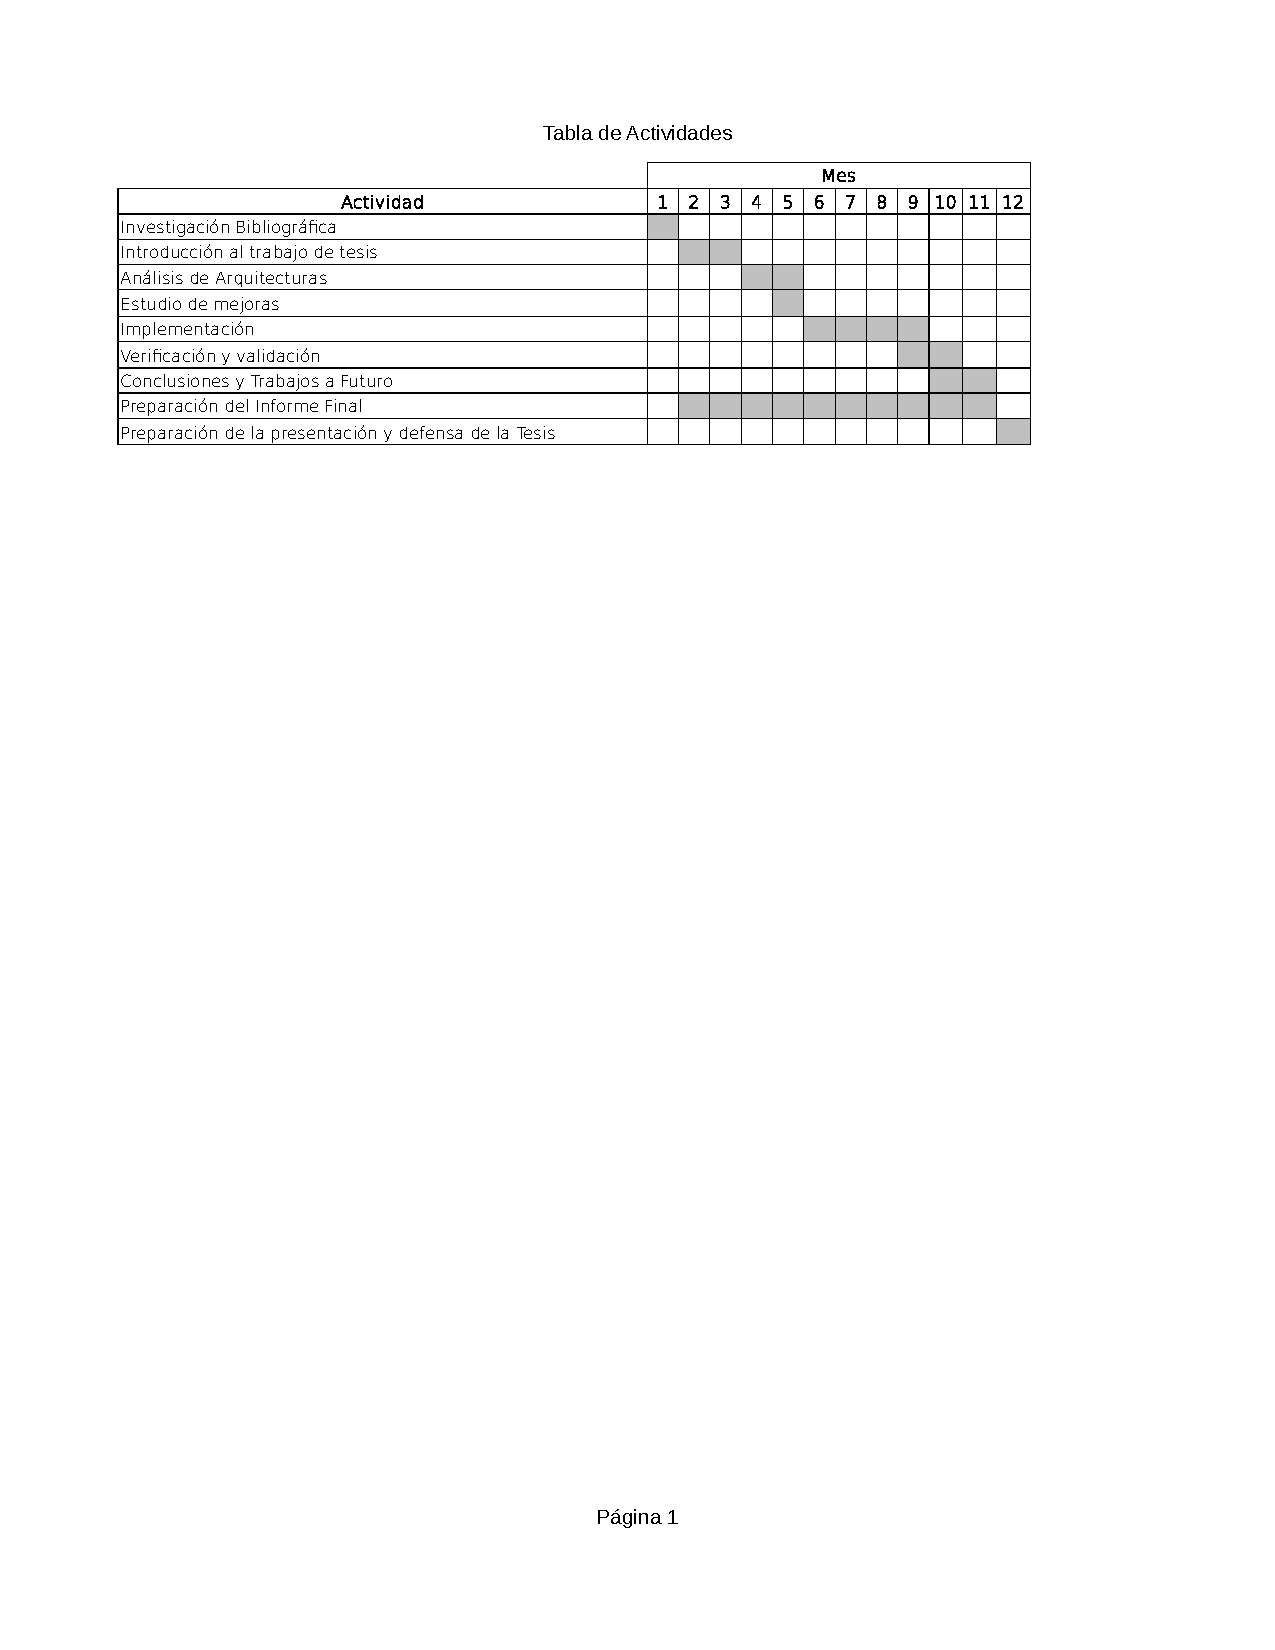
\includegraphics[trim = 20mm 200mm 20mm 25mm, clip, width=\textwidth]{tabla_actividades}
   \caption{Diagrama de las actividades a realizar por el tesista.}
\end{figure}

\newpage

\section{Bibliografía}

\begin{thebibliography}{99}

\bibitem{Mohammadi} Abbas Mohammadi \& Fadhel M. Ghannouchi, ``RF Transceiver Design for MIMO Wireless Communications'', Springer, p1-5, 2012.
\bibitem{Paulraj} Paulraj, A., Nabar, R., Gore, D., ``Introduction to Space-Time Wireless Communications''. Cambridge University Press, 2003.
\bibitem{Litva} John Litva \& Titus Kwok-Yeung Lo, ``Digital Beamforming in Wireless Communications'', Artech House, 1996.
\bibitem{Mohammadi2} Abbas Mohammadi \& Fadhel M. Ghannouchi, ``RF Transceiver Design for MIMO Wireless Communications'', Springer, p17-20, 2012.
\end{thebibliography}

\newpage

\signature{Buenos Aires}{Sr. Ignacio Lesser}{Tesista}{Ing. Nicolás Alvarez}{Ing. Octavio Alpago}{Prof. Adjunto, Director}{JTP. Interino, Co-director}

\end{document}
